
\documentclass{standalone}
\usepackage{tikz}
\usetikzlibrary{arrows.meta, positioning}
\usetikzlibrary{patterns,snakes}
\begin{document}

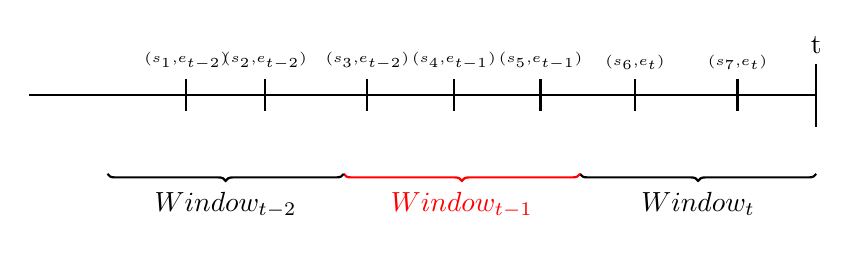
\begin{tikzpicture}
    \def\x{1}
  % Timeline
    \draw[thick] (0,0) -- (10,0);
    \draw[thick] (\x + 1,0.2) -- (\x + 1,-0.2);
    \node[above] at (\x+1, 0.2) {\tiny ($s_1$,$e_{t-2}$)};

 \draw[thick] (\x+2,0.2) -- (\x+2,-0.2);
    \node[above] at (\x+2, 0.2) {\tiny ($s_2$,$e_{t-2}$)};

 \draw[thick] (\x+3.3,0.2) -- (\x+3.3,-0.2);
    \node[above] at (\x+3.3, 0.2) {\tiny ($s_3$,$e_{t-2}$)};

 \draw[thick] (\x+4.4,0.2) -- (\x+4.4,-0.2);
    \node[above] at (\x+4.4, 0.2) {\tiny ($s_4$,$e_{t-1}$)};

 \draw[thick] (\x+5.5,0.2) -- (\x+5.5,-0.2);
    \node[above] at (\x+5.5, 0.2) {\tiny ($s_5$,$e_{t-1}$)};
    
    \draw[thick] (\x+6.7,0.2) -- (\x+6.7,-0.2);
    \node[above] at (\x+6.7, 0.2) {\tiny ($s_6$,$e_{t}$)};
 
    \draw[thick] (\x+8,0.2) -- (\x+8,-0.2);
    \node[above] at (\x+8, 0.2) {\tiny ($s_7$,$e_{t}$)};
 
    % End span
    \draw[thick] (10,0.4) -- (10,-0.4);
    \node[above] at (10,0.4) {t};

    \draw [
    thick,
    decoration={
        brace,
        mirror,
    },
    decorate
] (7, -1) -- (10, -1)
node [pos=0.5,anchor=north,yshift=-0.1cm] {$Window_t$};

    \draw [
    thick,
    red,
    decoration={
        brace,
        mirror,
    },
    decorate
] (4, -1) -- (7, -1)
    node [pos=0.5,anchor=north,yshift=-0.1cm] {$Window_{t-1}$};

    \draw [
    thick,
    decoration={
        brace,
        mirror,
    },
    decorate
] (1, -1) -- (4, -1)
    node [pos=0.5,anchor=north,yshift=-0.1cm] {$Window_{t-2}$};



\end{tikzpicture}

\end{document}
